
%-------------------------designed by zcf--------------
\documentclass[UTF8,a4paper,10pt]{ctexart}
\usepackage[left=3.17cm, right=3.17cm, top=2.74cm, bottom=2.74cm]{geometry}
\usepackage{amsmath}
\usepackage{graphicx,subfig}
\usepackage{float}
\usepackage{cite}
\usepackage{caption}
\usepackage{enumerate}
\usepackage{booktabs} %表格
\usepackage{multirow}
\usepackage{listings}
\lstset{
 columns=fixed,       
 numbers=left,                                        % 在左侧显示行号
 numberstyle=\tiny\color{gray},                       % 设定行号格式
 frame=none,                                          % 不显示背景边框
 backgroundcolor=\color[RGB]{245,245,244},            % 设定背景颜色
 keywordstyle=\color[RGB]{40,40,255},                 % 设定关键字颜色
 numberstyle=\footnotesize\color{darkgray},           
 commentstyle=\it\color[RGB]{0,96,96},                % 设置代码注释的格式
 stringstyle=\rmfamily\slshape\color[RGB]{128,0,0},   % 设置字符串格式
 showstringspaces=false,                              % 不显示字符串中的空格
 language=c,                                          % 设置语言
}
\newcommand{\tabincell}[2]{\begin{tabular}{@{}#1@{}}#2\end{tabular}}  %表格强制换行
%-------------------------字体设置--------------
\usepackage{times} 
\newcommand{\yihao}{\fontsize{26pt}{36pt}\selectfont}           % 一号, 1.4 倍行距
\newcommand{\erhao}{\fontsize{22pt}{28pt}\selectfont}          % 二号, 1.25倍行距
\newcommand{\xiaoer}{\fontsize{18pt}{18pt}\selectfont}          % 小二, 单倍行距
\newcommand{\sanhao}{\fontsize{16pt}{24pt}\selectfont}  %三号字
\newcommand{\xiaosan}{\fontsize{15pt}{22pt}\selectfont}        % 小三, 1.5倍行距
\newcommand{\sihao}{\fontsize{14pt}{21pt}\selectfont}            % 四号, 1.5 倍行距
\newcommand{\banxiaosi}{\fontsize{13pt}{19.5pt}\selectfont}    % 半小四, 1.5倍行距
\newcommand{\xiaosi}{\fontsize{12pt}{18pt}\selectfont}            % 小四, 1.5倍行距
\newcommand{\dawuhao}{\fontsize{11pt}{11pt}\selectfont}       % 大五号, 单倍行距
\newcommand{\wuhao}{\fontsize{10.5pt}{15.75pt}\selectfont}    % 五号, 单倍行距
%-------------------------章节名----------------
\usepackage{ctexcap} 
\CTEXsetup[name={,、},number={ \chinese{section}}]{section}
\CTEXsetup[name={(,)},number={\chinese{subsection}}]{subsection}
\CTEXsetup[name={,.},number={\arabic{subsubsection}}]{subsubsection}
%-------------------------页眉页脚--------------
\usepackage{fancyhdr}
\pagestyle{fancy}
\lhead{\kaishu \leftmark}
% \chead{}
\rhead{\kaishu 编译原理预备工作}%加粗\bfseries 
\lfoot{}
\cfoot{\thepage}
\rfoot{}
\renewcommand{\headrulewidth}{0.1pt}  
\renewcommand{\footrulewidth}{0pt}%去掉横线
\newcommand{\HRule}{\rule{\linewidth}{0.5mm}}%标题横线
\newcommand{\HRulegrossa}{\rule{\linewidth}{1.2mm}}
%-----------------------伪代码------------------
\usepackage[ruled]{algorithm2e}
%------------------------代码-------------------
\usepackage{xcolor} 
\usepackage{listings} 
\lstset{ 
breaklines,%自动换行
basicstyle=\small,
escapeinside=``,
keywordstyle=\color{ blue!70} \bfseries,
commentstyle=\color{red!50!green!50!blue!50},% 
stringstyle=\ttfamily,% 
extendedchars=false,% 
linewidth=\textwidth,% 
numbers=left,% 
numberstyle=\tiny \color{blue!50},% 
frame=trbl% 
rulesepcolor= \color{ red!20!green!20!blue!20} 
}
%------------超链接----------
\usepackage[colorlinks,linkcolor=black,anchorcolor=blue]{hyperref}
%------------------------TODO-------------------
\usepackage{enumitem,amssymb}
\newlist{todolist}{itemize}{2}
\setlist[todolist]{label=$\square$}
% for check symbol 
\usepackage{pifont}
\newcommand{\cmark}{\ding{51}}%
\newcommand{\xmark}{\ding{55}}%
\newcommand{\done}{\rlap{$\square$}{\raisebox{2pt}{\large\hspace{1pt}\cmark}}\hspace{-2.5pt}}
\newcommand{\wontfix}{\rlap{$\square$}{\large\hspace{1pt}\xmark}}
%------------------------水印-------------------
\usepackage{tikz}
\usepackage{xcolor}
\usepackage{eso-pic}

\newcommand{\watermark}[3]{\AddToShipoutPictureBG{
\parbox[b][\paperheight]{\paperwidth}{
\vfill%
\centering%
\tikz[remember picture, overlay]%
  \node [rotate = #1, scale = #2] at (current page.center)%
    {\textcolor{gray!80!cyan!30!magenta!30}{#3}};
\vfill}}}



%———————————————————————————————————————————正文———————————————————————————————————————————————
%----------------------------------------------
\begin{document}
\begin{titlepage}
    \begin{center}
    
\includegraphics[width=0.8\textwidth]{NKU.png}\\[1cm]    
    \textsc{\Huge \kaishu{\textbf{南\ \ \ \ \ \ 开\ \ \ \ \ \ 大\ \ \ \ \ \ 学}} }\\[0.9cm]
    \textsc{\huge \kaishu{\textbf{计算机学院和网络空间安全学院}}}\\[0.5cm]
    \textsc{\Large \textbf{编译原理实验报告}}\\[0.8cm]
    \HRule \\[0.9cm]
    { \LARGE \bfseries 预备工作一}\\[0.4cm]
    \HRule \\[2.0cm]
    \centering
    \textsc{\LARGE \kaishu{\ \ 陈宇轩 1911400}}\\[0.5cm]
    \textsc{\LARGE \kaishu{年级\ :\ 2019级}}\\[0.5cm]
    \textsc{\LARGE \kaishu{专业\ :\ 物联网工程}}\\[0.5cm]
    \textsc{\LARGE \kaishu{指导教师\ :\ 王刚}}\\[0.5cm]
    \vfill
    {\Large \today}
    \end{center}
\end{titlepage}
%-------------摘------要--------------
\newpage
\thispagestyle{empty}
\renewcommand{\abstractname}{\kaishu \sihao \textbf{摘要}}
    \begin{abstract}
    以gcc、llvm等为研究对象,利用各种方法,通过样例代码,简单的探究了代码处理过程中的
    各个步骤环节,包括预处理器、编译器、汇编器和链接器。
        \noindent  %顶格
        \textbf{\\\ 关键字:Complier , gcc , llvm , AST , RTL , Linker}\textbf{} \\\ \\\
    \end{abstract}
%----------------------------------------------------------------
\tableofcontents
%----------------------------------------------------------------
\newpage
\watermark{60}{10}{NKU}
\setcounter{page}{1}
\section{总体流程}
%——————————————————————————————————————
\subsection{预处理器}
C/C++代码的预处理器会在输入文件被编译之前根据预处理指令处理程序,主要包括文件包含、宏替换
和条件编译等,取决于预处理指令怎样书写。
\par
实验使用的代码如下:
\begin{lstlisting}
#include<stdio.h>
int main(){
    int i,n,f;
    scanf("%d",&n);
    i=2;
    f=1;
    while(i<=n){
        f=f*i;
        i=i+1;
    }
    printf("%d\n",f);
}
\end{lstlisting}
\par
使用gcc进行预编译处理,利用下列指令
\begin{lstlisting}
  gcc test.c -E -o test.i
\end{lstlisting}
将文件预编译结果输出到\href{run:./test/test.i}{test.i文件}中,
此时它仍然是一个C语言文件。gcc调用了C Pre-Processor完成了
例如替换include指令对应的头文件、添加行号和文件名标识等工作。
因为读入了stdio.h,预处理完成的文件变得十分庞大,观察一些内容就能知道,
C Pre-Processor在预处理程序时会先隐式的读取stdc-predef.h文件,
接着再根据stdio.h读入标准输入输出所需要的类型、宏和函数。
\par
具体的实现细节在官方给出的\href{run:./cpp.pdf}{说明文档}中有记录。
而\href{run:./test/test.i}{test.i}的内容就是编译器要处理的全部输入了。

%——————————————————————————————————————
\subsection{编译器}
\subsubsection{词法分析}
这一步要将源程序转换为有意义的单词(token)序列,编译器通过调用扫描器,让扫描器来完成这项工作。
命令
\begin{lstlisting}
  clang -E -Xclang -dump-tokens test.c
\end{lstlisting}
能够获得token序列,储存在\href{run:./test/token.txt}{token.txt文件}中:
\begin{lstlisting}
  typedef 'typedef'	 [StartOfLine]	Loc=</usr/lib/llvm-6.0/lib/clang/6.0.0/include/stddef.h:62:1>
  long 'long'	 [LeadingSpace]	Loc=</usr/lib/llvm-6.0/lib/clang/6.0.0/include/stddef.h:62:9 <Spelling=<built-in>:79:23>>
  unsigned 'unsigned'	 [LeadingSpace]	Loc=</usr/lib/llvm-6.0/lib/clang/6.0.0/include/stddef.h:62:9 <Spelling=<built-in>:79:28>>
  int 'int'	 [LeadingSpace]	Loc=</usr/lib/llvm-6.0/lib/clang/6.0.0/include/stddef.h:62:9 <Spelling=<built-in>:79:37>>
  identifier 'size_t'	 [LeadingSpace]	Loc=</usr/lib/llvm-6.0/lib/clang/6.0.0/include/stddef.h:62:23>
  semi ';'		Loc=</usr/lib/llvm-6.0/lib/clang/6.0.0/include/stddef.h:62:29>
  ...
\end{lstlisting}
\par
例如llvm处理的token序列结构形如:
\begin{lstlisting}
  属性   '内容'   ([位置])   定义位置
\end{lstlisting}
记录了每个单词的类型、“相貌”——它的值——和位置类型以及具体位置,以便之后的流程使用。
\par
这一阶段,源代码程序被输入到扫描器中,扫描器对源代码进行简单的词法分析,将源代码字符序列分割。
\par
lex是一种生成扫描器的工具,它工作的基本步骤是
\par
1.程序员编写文件,指定需要被扫描的词汇模式,lex生成的扫描器将根据这种模式进行工作
\par
2.对文件运行lex,生成扫描器的C代码
\par
3.编译、链接C代码,生成可执行文件
\par
lex的工作依赖于


\subsubsection{语法分析}
接下来,编译器要将单词序列处理为语法树。以gcc为例,使用命令
\begin{lstlisting}
  gcc fdump-tree-original-raw test.c
\end{lstlisting}
得到两个输出文件,\href{run:./test/a.out}{a.out}和\href{run:./test/test.c.003t.original}{test.c.003t.original},
a.out是test.c编译的可执行文件,test.c.003t.original就是获得的AST文件:
\begin{lstlisting}
  ;; Function main (null)
  ;; enabled by -tree-original
  
  @1      statement_list   0   : @2       1   : @3      
  @2      bind_expr        type: @4       vars: @5       body: @6      
  @3      return_expr      type: @4       expr: @7      
  @4      void_type        name: @8       algn: 8       
  @5      var_decl         name: @9       type: @10      scpe: @11     
                           srcp: test.c:3                size: @12     
                           algn: 32       used: 1       
  @6      statement_list   0   : @13      1   : @14      2   : @15     
                           3   : @16      4   : @17      5   : @18     
                           6   : @19      7   : @20      8   : @21     
                           9   : @22      10  : @23      11  : @24     
                           12  : @25      13  : @26   
  ...  
\end{lstlisting}
它的形式很容易让人联想到形如“如果你的答案是x,请跳至题目x”的一种测试选择题,
但是这里选项变成了分支,最终组成树的形式。
每一行是树的一个节点,行头是唯一的ID,接着是节点的属性,之后是子节点的ID和
父节点中它们各自的属性。

\subsubsection{语义分析}
标准委员会制订了语义标准,编译器将会根据这些标准、生成的符号表和语法树来检测源程序是否符合语义,
进行类型检查等。
\subsubsection{中间代码生成和优化}
这时大部分编译器已经生成了一组较源程序语言更加贴近底层,但是比二进制代码或汇编语言更加清晰,
更加便于分析逻辑结构的中间代码。它从源程序中提取出语义和语法结构,但并不依赖源程序语言或底层机器,
是沟通前端和后端的桥梁。
\par
gcc有三种不同的中间表示语言:AST/GENERIC(C前端)比较完善的表示了前端语言的信息;GIMPLE从AST转换而来,
是一种前端无关的中间表示;以及RTL(Register Transfer Language),它就是那个硬件无关以满足可复用性、
高度抽象以满足可优化性的中间语言。
\par
gcc在将源代码转化成中间代码的过程中会依次遍历这三种中间语言,AST已经在之前的语法分析阶段生成了,
并且由于不同的前端高级语言,gcc生成的AST是不同的,因此就需要转换为统一的GIMPLE形式。
\par
可以使用-fdump-tree-gimple、-fdump-rtl-all等flag来获得不同阶段的表达式,
也可以获得CFG和对应的dot图像。例如,我们对比AST和GIMPLE状态的代码:
如图\ref{fig:1}所示
\begin{figure}[H]
  \centering
  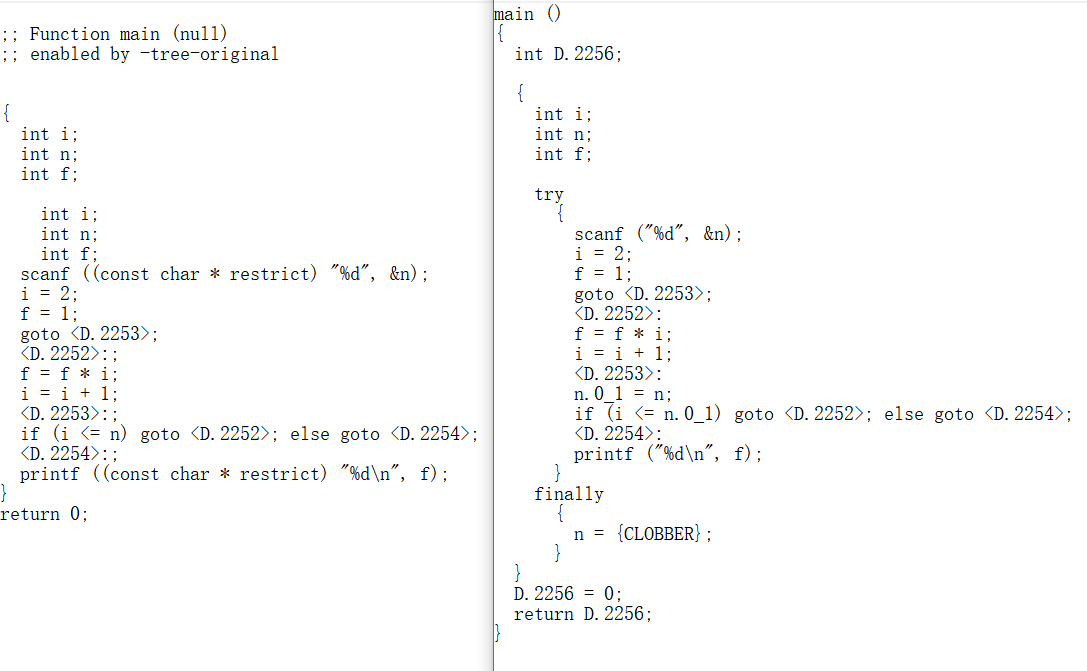
\includegraphics[scale=0.5]{generic_vs_gimple.png}
  \caption{GENERIC和GIMPLE}
  \label{fig:1}
\end{figure}
左边的文件来自\href{run:./test/all/test.c.003t.original}{test.c.003t.original},
右边的则是\href{run:./test/all/test.c.004t.gimple}{test.c.004t.gimple},这两个文件可以
通过使用-fdump-tree-all-graph这个flag得到。对比之下就会发现,GIMPLE表达式使用了
临时变量来储存计算中的中间值乃至返回值。除此之外,GIMPLE相比GENERIC还有一些其他优势,
诸如GENERIC是以树结构表示和储存的、GIMPLE前端无关而GENERIC相关、GIMPLE本质是线性代码序列,
能够更方便有效的进行后续的编译优化等。
\par
gcc在生成GIMPLE形式后,会先在这个层面上进行优化——低级化、构建CFG等一系列处理——
再转换为RTL形式。这些操作被称为GCC Pass,每一种pass完成一种处理,结果再作为下一个pass的输入。
\par
gcc描述pass的核心数据结构在passes.c文件中。优化pass分成4类,
分别是GIMPLE\_PASS、RTL\_PASS、SIMPLE\_IPA\_PASS、IPA\_PASS,
其中除了RTL\_PASS以RTL为处理对象,其他都以GIMPLE为对象。
通过-fdump-tree-all-graph这个flag可以生成具体的层次变化和对应的CFG流程图,
通过名字我们就能大致看出来gcc在这个阶段采取了怎样的优化。
\par
获得GIMPLE形式表达后,gcc后续还进行了许多处理步骤,保存在特定后缀的文件中,
每一遍的操作都属于IPA Pass(过程间优化),就像做菜时的手法,它们在各个过程间被适当的调用,
以完成一定的工作,也有可能被重复调用。
\par
上面谈到的有关pass的过程是借助Pass Manager完成的,它位于gcc源码中的passes.c、
tree-optimize.c、tree-pass.h文件中,根据passes.def中的定义来处理pass。
pass工作的原理就是让每一个pass定义一个结构,记录这个pass何时运行、怎样运行、
针对怎样的中间表达形式以及是否需要其他数据结构支持。在设置好pass以某种特定的规则运行以后,
Pass Manager就会保证它们按照规定执行。
\par
阅读这些中间文件——使用-fdump-tree-all-graph获得的一系列文档——
会发现这些处理中代码形式并没有太大变化,有一些关于返回值和计算中间量的存储和表示的变化,
但没有更多信息显得非常费解,这可能是因为源程序逻辑过于简单,以至于体现不出意图。
\par
更加简单的方式就是阅读说明文档和源码。\href{run:./gccint.pdf}{GCC Internals}中给出了
获得GIMPLE表示后,获得RTL之前,gcc做了哪些工作。此时调用的pass都属于Tree SSA Pass,
SSA是静态单赋值,是一种中间表示形式,每个名字在SSA中只被赋值一次。
\par
现在就能够知道一些文件处理的意义了,例如\href{run:./test/all/test.c.019t.fixup\_cfg1}{test.c.019t.fixup\_cfg1}
和\href{run:./test/all/test.c.020t.ssa}{test.c.020t.ssa}之间调用了
Enter static single assignment form处理文件,这个pass重写了程序使其成为SSA形式。
如图\ref{fig:2}
\begin{figure}[H]
  \centering
  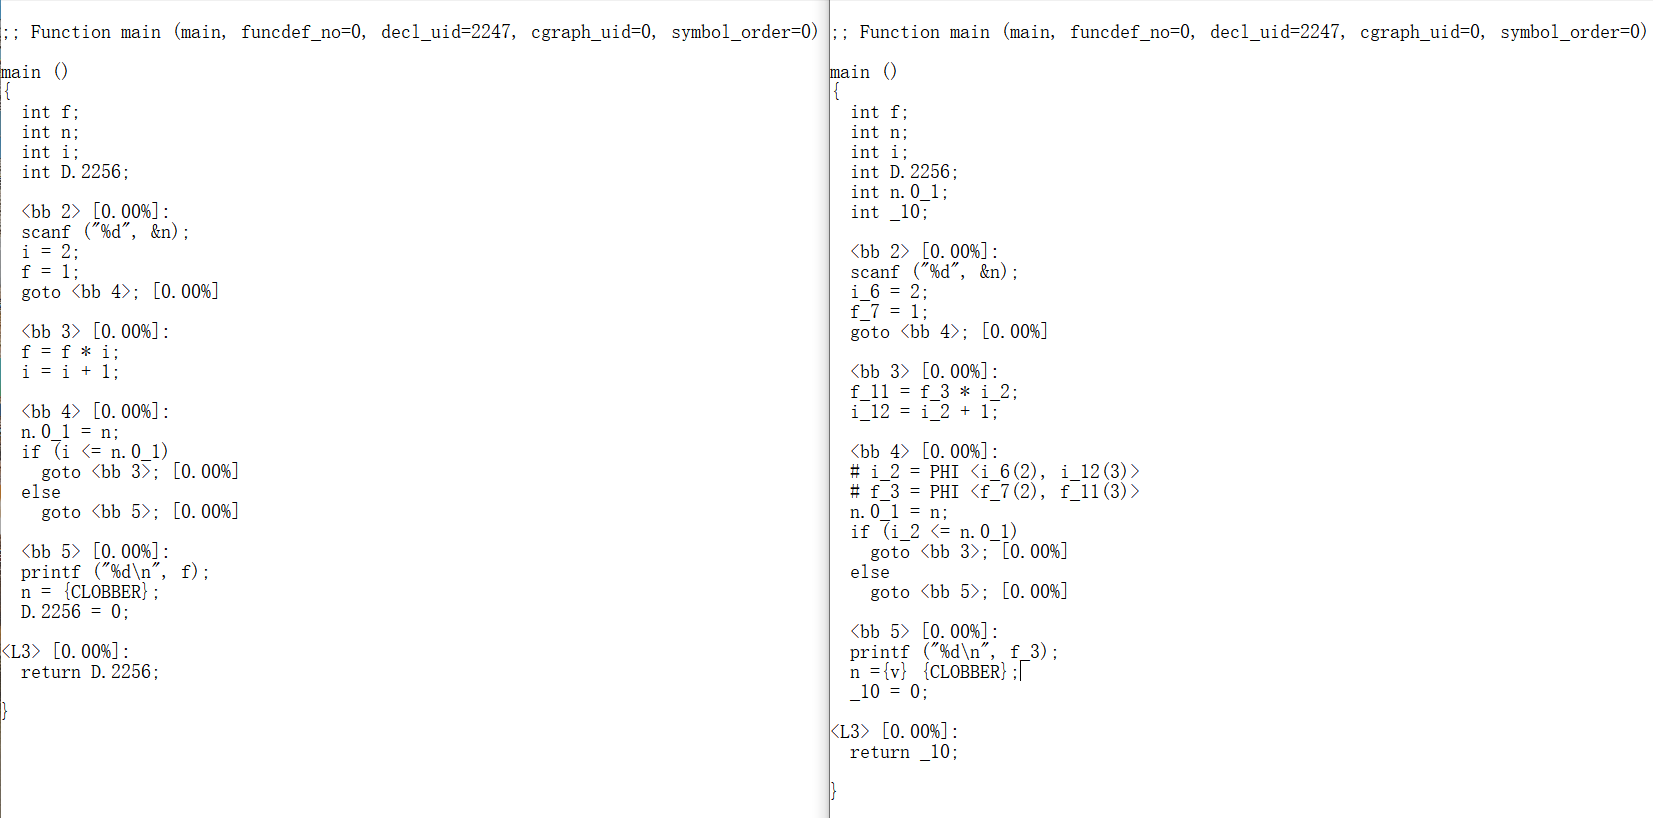
\includegraphics[scale=0.4]{cfg_vs_ssa.png}
  \caption{CFG和SSA}
  \label{fig:2}
\end{figure}
处理后所有is\_gimple\_reg变量
\footnote{无法寻址的堆栈变量}
都会以SSA\_NAME引用(后面加上了序号),为每个基本块按需加载PHI节点
\footnote{PHI节点由PHI指令实现。PHI指令是和基本块相关联的,它会根据上文BLOCK的内容决定取值}
(在基本块4中添加了PHI指令)
等。这个pass定义在tree-ssa.c中,由pass\_build\_ssa定义描述。
\footnote{令人失望的是,可能是由于这份gcc internal和发布在github上的gcc源码版本不同,我并没有找到源代码}
这样,我们就能一步步了解gcc在中间代码生成中做了什么。
\par
接下来是向RTL的转化,使用-fdump-rtl-all-graph,可以得到RTL形式下CFG的变化和对应dot图。
\par
使用-fdum-rtl-all可以得到RTL形式和在其上做的一系列优化,获得的第一个文件
\href{run:./test/rtl/test.c.229r.expand}{test.c.229r.expand}
给了关于GIMPLE形式是怎样转化为RTL形式的一些提示。
\begin{lstlisting}
;; Function main (main, funcdef_no=0, decl_uid=2247, cgraph_uid=0, symbol_order=0)

Partition 1: size 4 align 4
	f_3
Partition 0: size 4 align 4
	i_2
Partition 2: size 4 align 4
	n

;; Generating RTL for gimple basic block 2

;; Generating RTL for gimple basic block 3

;; Generating RTL for gimple basic block 4

;; Generating RTL for gimple basic block 5

;; Generating RTL for gimple basic block 6

try_optimize_cfg iteration 1

Merging block 3 into block 2...
Merged blocks 2 and 3.
Merged 2 and 3 without moving.
Merging block 7 into block 6...
Merged blocks 6 and 7.
Merged 6 and 7 without moving.
Removing jump 36.
Merging block 8 into block 6...
Merged blocks 6 and 8.
Merged 6 and 8 without moving.

try_optimize_cfg iteration 2
...
\end{lstlisting}
代码的格式和最初的c代码也没有太大区别,声明了函数和三个变量,接下来是一段声明,
“为gimple基本块x建立RTL”,虽然没有具体细节,但是从中可以知道从GIMPLE向RTL转换
是以基本块为单位的。接着是对已经转化为RTL形式,但仍保持着原来基本块结构的代码的优化,
文件中记录了对基本块、跳转语句的一些操作。
\href{run:./gccint.pdf}{GCC Internals}中记录了RTL的pass的简短介绍和如何在源码中找到它们。
\par
代码的RTL表示被称为INSN,它和之前的形式看起来完全不同了。有些INSN表示实际的指令,
有些代表switch语句的跳转表,有些表示程序跳转所对应的标号,还有一些可以表示各种不同的声明信息。
所有的INSN被一个双向链表所链接。
\par
INSN的具体格式如下:
\\
(insn\ 第1个操作数\ 第2个操作数\  第3个操作数\ 第4个操作数...第7操作数)
\par
在一个函数中,每一个INSN都具有唯一的标识ID(整数),也就是第一个操作数,
同时,每个INSN还包含了它的前驱(第二个操作数)和后继(第三个操作数)。第四个操作数表示
该条指令序列所在的基本块,这可以从列举的第二条指令看出。
第五个操作数就是这个INSN的主体了,描述了该INSN的RTL指令模版。第六个操作数是INSN的代码,
即该INSN描述动作的对应指令的索引值。第七操作数未使用。
\begin{lstlisting}
  ...
  (note 1 0 4 NOTE_INSN_DELETED)
  (note 4 1 2 2 [bb 2] NOTE_INSN_BASIC_BLOCK)
  (note 2 4 3 2 NOTE_INSN_FUNCTION_BEG)
  (insn 3 2 6 2 (parallel [
              (set (mem/v/f/c:DI (plus:DI (reg/f:DI 82 virtual-stack-vars)
                          (const_int -8 [0xfffffffffffffff8])) [1 D.2259+0 S8 A64])
                  (unspec:DI [
                          (const_int 40 [0x28])
                      ] UNSPEC_SP_TLS_SET))
              (set (scratch:DI)
                  (const_int 0 [0]))
              (clobber (reg:CC 17 flags))
          ]) "test.c":2 -1
       (nil))
  ...
  \end{lstlisting}
这是\href{run:./test/rtl/test.c.229r.expand}{test.c.229r.expand}开头的几个INSN,
即使不知道RTL语言的细节,通过INSN中的描述和DI等关键字,也能够猜出大概是在完成完善基本块、
分配堆栈等任务。
\par
经过gcc对中间代码的一遍遍优化,最终我们能得到面向后端的汇编语言。

\subsubsection{代码生成}
上面关于中间语言的过程隐藏的很隐蔽,直接以预处理后的\href{run:./test/test.i}{test.i}
文件作为输入
\begin{lstlisting}
  gcc test.i -S -o test_x86.S #生成 x86 格式目标代码
  arm-linux-gnueabihf-gcc test.i -S -o test_arm.S # 生成 arm 格式目标代码
\end{lstlisting}
我们就能获得arm和x86格式的目标语言格式代码\href{run:./test/test\_x86.S}{test\_x86.S}和
\href{run:./test/test\_arm.S}{test\_arm.S},上面的工作都完成了。

\subsubsection{gcc的优化级别}
gcc提供了编译时的优化选项供我们选择,分为从O0到O3的级别,和Os、Og、Ofast等特殊级别。
在编译时加入这些选项可以粗略的查看gcc提供了怎样的优化。
\begin{lstlisting}
  gcc -O0 -o o0.S -S -masm=att test.i  #获得O0级别输出
  gcc -O1 -o o1.S -S -masm=att test.i  #获得O1级别输出
\end{lstlisting}
其中O0不做任何优化,也是默认的编译选项,\href{run:./test/o0.S}{o0.S}的内容就是gcc直接获得的汇编代码。
它和执行O1级优化获得的\href{run:./test/o1.S}{o1.S}的区别在于,O1优化试图消耗较少的编译时间,
以获得一定的优化,它主要对代码的分支、常量以及表达式等进行优化。相较于O0不做任何优化,
它会延迟栈的弹出时间,简化连续的、条件相关的比较语句的跳转,执行循环优化等。O2优化
则会尝试更多的寄存器级和指令级的优化,占用更多的编译时间,O3自然更加复杂。随着优化等级的
一步步上升,它们消耗的时间和资源,以及最终获得的代码复杂程度都会上升。通过阅读
\href{run:./gcc.pdf}{GCC MANUAL}p151开始的关于编译优化的内容,我们能获得更多信息。


\subsection{汇编器}
汇编器属于编译器的后端,这里将要输出对应的机器代码。它的工作是生成可重定位的机器代码,
为此,汇编器需要翻译程序中那些能够完成自己任务的代码块,通常还需要进行优化,使得最终
链接器把所有文件整合生成可执行文件的过程和结果更优。汇编器同样有一定的工作流程,
以Beignet的后端部分为例,它分为四个步骤:

\subsubsection{指令选择}
这一阶段中,汇编器会非常简单、快速、草率的生成指令序列。这看起来很像之前中间代码生成时
做的事:先翻译,再优化。
此时我们会在尽可能控制成本的基础上,把每个基本块翻成一串ISA指令组,而做法就是简单的把每一句
中间语言指令不计数量地翻译成ISA指令去完成功能。在这个过程中,事实上我们输出的是一些
SelectionInstruction对象,它能够通过编码函数一对一的翻译为ISA,并且它仍然使用未定位的
虚拟寄存器和其元组。

\subsubsection{寄存器分配}
它分为两个步骤:
\par
1.为需要的指令处理向量。步骤一需要扫描所有需要被发射的向量。为了避免不同向量使用同一个寄存器可能引发的冲突和干扰,
Beignet把向量从小到大排列并按顺序分配,还识别了包含在较大向量中的子向量保留。
\par
2.执行寄存器分配。步骤二就是将每个虚拟寄存器和物理寄存器相关联。寄存器显然不能任意分配,
我们需要考虑各种策略和机制保证它们在之后的过程中不会出错。

\subsubsection{指令调度}
引入寄存器以后,指令的执行顺序很有可能需要被做出调整,这部分优化不能提前完成。我们可以想象
汇编器以调用pass的形式对指令进行遍历和优化。

\subsubsection{指令编码}
这一步骤就是将代码最终在机器上运行可能遇到的,包括基于硬件基础的问题解决,成为真正的机器码。

\subsubsection{一个例子}
还是举开头的C代码为例,获得汇编器处理后的文件,并用反汇编查看其代码
\begin{lstlisting}
  gcc -c -o test.o test.c     #获得汇编后的可重定位文件test.o
  objdump -d test.o > test-anti-obj.S     #反汇编查看获得的文件
  nm test.o > test-nm-obj.txt      #列出文件中的符号信息(定义出的函数、全局变量等)
\end{lstlisting}
我们获得了\href{run:./test/test-anti-obj.S}{test-anti-obj.S}和
\href{run:./test/test-nm-obj.txt}{test-nm-obj.txt},分别是反汇编指令和name指令的结果。
\begin{lstlisting}
  0000000000000000 <main>:
  0:	55                   	push   %rbp
  1:	48 89 e5             	mov    %rsp,%rbp
  4:	48 83 ec 20          	sub    $0x20,%rsp
  8:	64 48 8b 04 25 28 00 	mov    %fs:0x28,%rax
  f:	00 00 
 11:	48 89 45 f8          	mov    %rax,-0x8(%rbp)
 15:	31 c0                	xor    %eax,%eax
 17:	48 8d 45 ec          	lea    -0x14(%rbp),%rax
 1b:	48 89 c6             	mov    %rax,%rsi
 1e:	48 8d 3d 00 00 00 00 	lea    0x0(%rip),%rdi        # 25 <main+0x25>
 25:	b8 00 00 00 00       	mov    $0x0,%eax
 2a:	e8 00 00 00 00       	callq  2f <main+0x2f>
 2f:	c7 45 f0 02 00 00 00 	movl   $0x2,-0x10(%rbp)
 36:	c7 45 f4 01 00 00 00 	movl   $0x1,-0xc(%rbp)
 3d:	eb 0e                	jmp    4d <main+0x4d>
 3f:	8b 45 f4             	mov    -0xc(%rbp),%eax
 42:	0f af 45 f0          	imul   -0x10(%rbp),%eax
 46:	89 45 f4             	mov    %eax,-0xc(%rbp)
 49:	83 45 f0 01          	addl   $0x1,-0x10(%rbp)
 4d:	8b 45 ec             	mov    -0x14(%rbp),%eax
 50:	39 45 f0             	cmp    %eax,-0x10(%rbp)
 53:	7e ea                	jle    3f <main+0x3f>
 55:	8b 45 f4             	mov    -0xc(%rbp),%eax
 58:	89 c6                	mov    %eax,%esi
 5a:	48 8d 3d 00 00 00 00 	lea    0x0(%rip),%rdi        # 61 <main+0x61>
 61:	b8 00 00 00 00       	mov    $0x0,%eax
 66:	e8 00 00 00 00       	callq  6b <main+0x6b>
 6b:	b8 00 00 00 00       	mov    $0x0,%eax
 70:	48 8b 55 f8          	mov    -0x8(%rbp),%rdx
 74:	64 48 33 14 25 28 00 	xor    %fs:0x28,%rdx
 7b:	00 00 
 7d:	74 05                	je     84 <main+0x84>
 7f:	e8 00 00 00 00       	callq  84 <main+0x84>
 84:	c9                   	leaveq 
 85:	c3                   	retq  
\end{lstlisting}
即使不懂得汇编语言,第一眼我们就能发现它较之前利用-S参数只编译生成的
\href{run:./test/test.S}{test.S}文件要紧凑,
同时至少能注意到的是,机器指令中所有的跳转地址都定义为<main+0xXX>的形式。
\par
再看nm指令获得的输出
\begin{lstlisting}
                  U _GLOBAL_OFFSET_TABLE_
                  U __isoc99_scanf
0000000000000000  T main
                  U printf
                  U __stack_chk_fail
\end{lstlisting}
这里U和T都是符号类型,U表示未定义,需从其他对象文件链接进来,可以看出都是外部的全局偏移表和库函数等;
T表示符号在代码段中,也就是main函数。这些在链接完成后想必会有所变化。

\subsection{链接器、加载器}
链接器的工作,是确保此前文件中的依赖关系是正确的,将给定的目标文件集合拼接打包,最终对其进行重定位。
\par
还是看例子。链接汇编后的.o文件并对其执行反汇编等操作
\begin{lstlisting}
  gcc -o TEST test.o
  objdump -d TEST > TEST-anti-obj.S
  nm TEST > TEST-nm-obj.txt
\end{lstlisting}
最终我们获得了可执行文件\href{run:./test/TEST}{TEST},和对它执行反汇编和name指令获得的输出
\href{run:./test/TEST1-anti-obj.S}{TEST1-anti-obj.S}、
\href{run:./test/TEST1-nm-obj.txt}{TEST1-nm-obj.txt}。现在反汇编文件已经大到不适合放进
文中了,这当然是因为程序运行所需要的所有代码现在都被链接进了TEST中,它们各自成块,彼此调用。
nm指令现在获得的部分输出如下:
\begin{lstlisting}
  ...
  0000000000200fa8 d _GLOBAL_OFFSET_TABLE_
                   w __gmon_start__
  000000000000082c r __GNU_EH_FRAME_HDR
  00000000000005a8 T _init
  0000000000200db0 t __init_array_end
  0000000000200da8 t __init_array_start
  0000000000000820 R _IO_stdin_used
                   U __isoc99_scanf@@GLIBC_2.7
                   w _ITM_deregisterTMCloneTable
                   w _ITM_registerTMCloneTable
  0000000000000810 T __libc_csu_fini
  00000000000007a0 T __libc_csu_init
                   U __libc_start_main@@GLIBC_2.2.5
  000000000000071a T main
                   U printf@@GLIBC_2.2.5
  0000000000000680 t register_tm_clones
                   U __stack_chk_fail@@GLIBC_2.4
  0000000000000610 T _start
  0000000000201010 D __TMC_END__  
\end{lstlisting}
果然,现在文件中有大量的符号,它们原本存放在库文件或其他地方,现在被集中到了可执行文件中。
\par
但是,如果在链接时使用-static参数,再执行同样操作,我们获得的文件
\footnote{\href{run:./test/staticTEST-anti-obj.S}{staticTEST-anti-obj.S}、
\href{run:./test/staticTEST-nm-obj.txt}{staticTEST-nm-obj.txt}}
的大小会比现在恐怖的多,这就是静态链接和动态链接的区别,是它们在对库的取舍
——我全都要还是一会儿来拿——和链接时机的选择——现在就执行和开始执行时再说——的不同造成的。

%----------------------------------------------------------------
\section{总结}


%----------------------------------------------------------------
\newpage
\bibliographystyle{plain}
\bibliography{references} 
\end{document}
